% PQ-RNS: Hybrid Post-Quantum Profile for the Reticulum Network Stack
%
% Build: latexmk -pdf pq-rns.tex
\documentclass[11pt,a4paper]{article}
\usepackage{../shared/luxcover}
\usepackage[utf8]{inputenc}
\usepackage[T1]{fontenc}
\usepackage{amsmath,amssymb,amsfonts}
\usepackage{graphicx}
\usepackage{hyperref}
\usepackage{booktabs}
\usepackage{listings}
\usepackage{xcolor}
\usepackage{tikz}
\usepackage{float}
\usepackage{enumitem}
\usepackage{array}
\usepackage{tabularx}
\input{../shared/lstlang}
\usetikzlibrary{arrows.meta,positioning,shapes.geometric,fit,calc}

\hypersetup{colorlinks=true,linkcolor=black,citecolor=blue,urlcolor=blue}

\lstset{
  basicstyle=\ttfamily\scriptsize,
  breaklines=true,
  frame=single,
  numbers=left,
  numberstyle=\tiny\color{gray},
  keywordstyle=\color{blue!70!black}\bfseries,
  commentstyle=\color{green!50!black}\itshape,
  stringstyle=\color{red!60!black},
  showstringspaces=false,
}

\title{\textbf{PQ-RNS}\\
       \large A hybrid post-quantum profile for the\\
       Reticulum Network Stack (LP-9701)}
\author{Lux Industries Inc.\\
        \texttt{security@lux.network}}
\date{Draft \today}

\begin{document}
\maketitle

\begin{abstract}
The Reticulum Network Stack (RNS)~\cite{rns-manual,rns-repo} is a
cryptography-based mesh-networking stack designed by Mark Qvist for
LoRa, packet radio, KISS modems, serial lines, free-space optical
links, and any other half-duplex carrier with at least 5\,bps and a
500-byte MTU. RNS provides initiator-anonymous, coordination-less,
multi-hop transport with end-to-end encryption and unforgeable delivery
acknowledgements, completely without IP. Its native cryptographic suite
is classical: 256-bit Curve25519 keysets (X25519 for ECDH, Ed25519 for
signatures), AES-256-CBC + HMAC-SHA-256 in a Fernet-style token format,
SHA-256 and SHA-512 for hashing, and HKDF for key derivation. That
suite is well-engineered and well-implemented, but Curve25519 is broken
by a sufficiently large quantum computer: a passive recorder today can
decrypt every session retrospectively when one becomes available.
\textbf{PQ-RNS} is the Lux profile (LP-9701~\cite{lp9701}) that adds a
hybrid post-quantum layer on top of classical RNS without forking the
protocol: classical RNS identity (Ed25519 + X25519) remains the
on-the-wire baseline; ML-KEM-768 (FIPS~203~\cite{fips203}) and
ML-DSA-65 (FIPS~204~\cite{fips204}) extensions ride alongside in
capability-negotiated announce frames. Sessions derive their AES-256
key from $\textsf{HKDF}(\textsf{X25519 shared}\,\|\,\textsf{ML-KEM shared})$
so retrospective decryption requires breaking both legs.
This profile is the transport that PQSAFE-IL5-HYBRID-v1 envelopes ride
when IP is unavailable: contested electromagnetic environments,
disaster-recovery, off-grid mesh, LoRa, and amateur-radio packet
networks.
\end{abstract}

\tableofcontents

% ===========================================================================
\section{Why RNS}
\label{sec:why-rns}

Most post-quantum work assumes a TCP/IP carrier. RNS is the answer when
the carrier itself is contested:

\begin{itemize}[leftmargin=*,itemsep=0pt]
\item \textbf{No IP needed.} RNS runs on any half-duplex medium with
  $\geq$5\,bps and an MTU of $\geq$500 bytes. Wired Ethernet, WiFi,
  TCP/UDP, serial, KISS, AX.25, RNode LoRa, free-space optical, and
  custom modems are all first-class carriers.
\item \textbf{Coordination-less globally unique addressing.} A node's
  address \emph{is} the hash of its long-term Curve25519 identity --
  no DNS, no DHCP, no IANA. Two nodes that have never seen each other
  before still can address each other.
\item \textbf{Initiator anonymity.} RNS packets carry no source
  address. The recipient knows who can decrypt; the network doesn't
  learn who sent.
\item \textbf{Self-configuring multi-hop transport.} The protocol
  picks paths through any mixture of mediums automatically. A laptop
  on WiFi can reach a sensor on LoRa via a Raspberry Pi gateway with
  no operator configuration.
\item \textbf{Resilient on intermittent / hostile networks.}
  Single-byte amplification attacks and packet-loss-induced
  amplification (TCP's pathologies) don't apply; RNS is designed for
  high packet loss.
\item \textbf{Low cost of keeping links open.} A maintained RNS link
  costs roughly 0.44\,bits/second of overhead. A full encrypted +
  authenticated link setup costs 297 bytes across 3 packets.
\end{itemize}

These properties make RNS the right transport for off-grid mesh, disaster
recovery, contested EW environments, and IL5/CUI traffic over media
that don't support TLS at all. Lux uses RNS as a peer of TCP/IP for
validator-to-validator gossip in degraded conditions and as the
underlay for PQSAFE envelopes when those envelopes are exchanged
out-of-band of the broader internet.

\subsection{Authoritative RNS reference}

The Python reference implementation~\cite{rns-repo} is the
authoritative protocol definition. The maintainer's identity hash is
\texttt{bc7291552be7a58f361522990465165c}. A protocol implementation
is Reticulum if and only if it interoperates with that reference. The
Lux PQ profile is a strict layer atop the reference: capability
extension, not a fork.

% ===========================================================================
\section{Native RNS cryptographic suite (baseline)}
\label{sec:rns-native}

The native RNS suite, taken verbatim from the reference manual and
reference implementation, is:

\begin{table}[H]
\centering
\small
\begin{tabularx}{\linewidth}{l X}
\toprule
\textbf{Component} & \textbf{Native primitive (classical)} \\
\midrule
Identity (signing) & Ed25519 (256 bits) \\
Identity (KEX) & X25519 (256 bits) \\
Session encryption & AES-256-CBC + PKCS7 padding \\
Authenticated tag & HMAC-SHA-256 \\
KDF & HKDF-SHA-256 \\
IVs & 16 bytes from \texttt{os.urandom()} \\
Hash & SHA-256, SHA-512 \\
Token format & Fernet-style (no version / timestamp metadata) \\
\bottomrule
\end{tabularx}
\caption{Native RNS primitives. Source: \texttt{markqvist/Reticulum}
\texttt{Cryptographic Primitives} section.}
\end{table}

This suite is secure against classical adversaries to roughly the
128-bit level (limited by the curve), with AEAD-equivalent integrity
through the Encrypt-then-MAC composition. It is \emph{not}
post-quantum: Curve25519 falls to Shor's algorithm.

\subsection{Forward secrecy in native RNS}

Native RNS already provides per-link forward secrecy: every link
establishment runs a fresh X25519 ECDH between ephemeral keys, and the
derived AES-256-CBC + HMAC-SHA-256 keys are scoped to that link. A
compromise of either side's long-term Curve25519 identity does not
permit retrospective decryption of recorded link traffic, because the
ephemeral half is gone.

PQ-RNS preserves this property and extends it to the quantum
adversary.

% ===========================================================================
\section{PQ-RNS: the Lux profile}
\label{sec:pq-rns}

\subsection{Goals}

\begin{enumerate}[leftmargin=*,itemsep=0pt]
\item \textbf{Quantum-safe confidentiality} for every PQ-RNS link, even
  against a passive recorder with a future CRQC.
\item \textbf{Quantum-safe authenticity} for every PQ-RNS identity.
\item \textbf{Backward compatibility} with native RNS: mixed networks
  (PQ-capable and classical-only peers) coexist; PQ-required nodes
  cleanly refuse classical-only counterparties without breaking the
  rest of the mesh.
\item \textbf{Zero protocol fork.} PQ-RNS rides as a capability
  extension; the reference RNS implementation is the source of truth.
\item \textbf{Bandwidth-conscious.} Mesh and LoRa carriers measure in
  bits per second. The PQ extension must amortise its handshake cost
  across many sessions; per-packet overhead should not grow.
\end{enumerate}

\subsection{Cryptographic stack}

\begin{table}[H]
\centering
\small
\begin{tabularx}{\linewidth}{l X X}
\toprule
\textbf{Purpose} & \textbf{Native RNS (classical)} & \textbf{PQ-RNS extension (hybrid)} \\
\midrule
Identity signing & Ed25519 & Ed25519 + ML-DSA-65 (FIPS~204) \\
Key exchange & X25519 & X25519 + ML-KEM-768 (FIPS~203) \\
Session encryption & AES-256-CBC + HMAC-SHA-256 & AES-256-CBC + HMAC-SHA-256 (unchanged) \\
Key derivation & HKDF-SHA-256 & HKDF-SHA-256 over hybrid secret \\
Long-term identity & 64-byte (Ed25519 || X25519) & $\sim$3.2 KiB (Ed25519 || X25519 || ML-DSA-65 || ML-KEM-768) \\
\bottomrule
\end{tabularx}
\caption{PQ-RNS hybrid stack vs.\ native RNS.}
\end{table}

The session encryption and integrity stay AES-256-CBC + HMAC-SHA-256
verbatim. AES-256 retains 128-bit effective security against Grover;
HMAC-SHA-256 retains comparable strength. The hybrid extension lives
at the identity and key-exchange layers, where the classical
primitives fail to a CRQC.

\subsection{Identity layout}

A PQ-RNS identity is a sequence of four key blobs:

\begin{lstlisting}[caption={Hybrid identity wire layout.}]
PQ-RNS Identity ::= {
  type:           u16 = 0x0002          // 0x0001 = classical, 0x0002 = hybrid
  ed25519_pub:    [u8;  32]
  x25519_pub:     [u8;  32]
  mldsa65_pub:    [u8; 1952]            // FIPS 204 ML-DSA-65 pubkey
  mlkem768_pub:   [u8; 1184]            // FIPS 203 ML-KEM-768 pubkey
  fingerprint:    [u8;  16]             // SHA-256 truncated, same as native
}
\end{lstlisting}

The native 16-byte fingerprint is preserved -- it is computed over the
\emph{whole} identity blob (including the PQ keys), so a hybrid node's
address is stable, globally unique, and observably distinct from a
classical-identity hash.

\subsection{Hybrid link establishment}

Native RNS establishes an encrypted link in three packets totalling
297 bytes. PQ-RNS keeps the 3-packet shape; sizes grow.

\begin{lstlisting}[caption={Hybrid link-establishment packets.}]
LinkRequest ::= {
  initiator_id_hash:  [u8; 16]
  initiator_eph_x25519:  [u8; 32]
  initiator_eph_mlkem768_ct: [u8; 1088]  // ct to responder's static MLKEM
  hybrid_capability_flags: u16
  ed25519_sig(over above): [u8; 64]
  mldsa65_sig(over above): [u8; 3309]
}                                          // ~4.5 KiB

LinkAccept ::= {
  responder_eph_x25519: [u8; 32]
  responder_eph_mlkem768_ct: [u8; 1088]   // ct to initiator's eph MLKEM
  responder_ack_hmac: [u8; 32]            // HMAC over derived key
  ed25519_sig: [u8; 64]
  mldsa65_sig: [u8; 3309]
}                                          // ~4.5 KiB

LinkActivate ::= {
  initiator_ack_hmac: [u8; 32]
  -- no signatures: the link is already authenticated
}                                          // 32 bytes
\end{lstlisting}

The derived session key is

$$K_\text{link} = \textsf{HKDF-SHA-256}\bigl(
\textsf{X25519}_\text{eph-eph}\,\|\,
\textsf{ML-KEM-768}_\text{eph-eph},\
\text{info}=H(\text{transcript})\bigr)$$

where the transcript is the concatenation of all three packet payloads
up to the AEAD layer. The HKDF info-string binding makes the key
context-locked: a replay of LinkRequest with a different LinkAccept
derives a different key, so an attacker cannot graft halves of two
sessions together.

\subsection{Ephemeral keys, perfect forward secrecy}

Both halves of the KEM are ephemeral:

\begin{itemize}[leftmargin=*,itemsep=0pt]
\item Each peer generates a fresh X25519 keypair and a fresh
  ML-KEM-768 keypair per link.
\item The two ephemeral private keys are zeroed once $K_\text{link}$
  is derived.
\item A future compromise of either long-term key (Ed25519 or
  ML-DSA-65) lets the adversary impersonate the identity going
  forward, but cannot decrypt recorded link traffic.
\item Retrospective decryption requires breaking \emph{both}
  ephemeral keys -- one classical, one lattice -- for every recorded
  link. This is the hybrid PFS contract.
\end{itemize}

\subsection{AEAD over PQ-RNS}

Native RNS uses Encrypt-then-MAC: AES-256-CBC + HMAC-SHA-256 in a
Fernet-style token. PQ-RNS keeps this exact construction. We do not
switch to AES-GCM because the native Fernet framing is part of the
on-wire RNS protocol; replacing it would break interoperability with
the reference implementation. The integrity tag length, padding, and
sequencing are unchanged. The only difference is the key material:
$K_\text{link}$ derives from the hybrid secret, not the classical-only
X25519 secret.

If a future RNS revision adopts a true AEAD (e.g., AES-GCM with
sequence-numbered nonces, or ChaCha20-Poly1305), the PQ profile
inherits that change immediately -- the PQ extension affects the key
derivation only, not the AEAD construction.

% ===========================================================================
\section{Wire-format growth}
\label{sec:size}

The cost of going from native RNS to PQ-RNS is approximately one
order of magnitude in handshake bytes. Steady-state link cost is
unchanged.

\begin{table}[H]
\centering
\small
\begin{tabular}{l r r r}
\toprule
\textbf{Component} & \textbf{Classical} & \textbf{Hybrid} & \textbf{$\Delta$} \\
\midrule
Public identity & 64 B & $\sim$3.2 KiB & +3.1 KiB \\
Signature (one) & 64 B & $\sim$2.5 KiB & +2.4 KiB \\
Key exchange ct (one) & 32 B & $\sim$1.2 KiB & +1.1 KiB \\
LinkRequest packet & $\sim$96 B & $\sim$4.5 KiB & +4.4 KiB \\
LinkAccept packet & $\sim$64 B & $\sim$4.5 KiB & +4.4 KiB \\
LinkActivate packet & 32 B & 32 B & 0 B \\
\midrule
\textbf{Total handshake} & $\sim$192 B (3 pkts) & $\sim$9 KiB (3 pkts) & +8.8 KiB \\
Steady-state per-packet overhead & 0.44 bps & 0.44 bps & 0 \\
\bottomrule
\end{tabular}
\caption{Wire-format growth from native RNS to PQ-RNS.}
\end{table}

\subsection{Bandwidth implications}

\begin{itemize}[leftmargin=*,itemsep=0pt]
\item \textbf{Ethernet / WiFi / TCP-over-IP.} 9 KiB handshake at
  100\,Mbps takes 0.7\,ms. Irrelevant.
\item \textbf{KISS / serial 9600 baud.} 9 KiB takes $\sim$7.5\,s.
  Tolerable for one-off link setup; amortised across many requests
  on the link.
\item \textbf{LoRa @ SF7BW125 (5470 bps usable).} 9 KiB takes
  $\sim$14\,s of channel time. Acceptable for a one-shot file drop;
  for streaming workloads, use a smaller hybrid (X25519-only or
  ML-KEM-only) or move to a faster medium for the handshake and
  re-engage on the link.
\item \textbf{LoRa @ SF12BW125 (250 bps).} 9 KiB takes
  $\sim$5 minutes. PQ-RNS in this regime is for low-rate command \&
  control only; consider a pre-shared key (PSK) hybrid mode where
  the long-term identity is exchanged out-of-band and only ephemeral
  KEMs ride on the channel.
\item \textbf{Free-space optical / packet-radio 1200 baud.}
  $\sim$60\,s. Practical for low-frequency link refresh.
\end{itemize}

\subsection{PSK-hybrid mode for low-bandwidth carriers}

For sub-1\,Kbps carriers, PQ-RNS offers a PSK-hybrid mode:

\begin{itemize}[leftmargin=*,itemsep=0pt]
\item Long-term ML-KEM-768 public keys are exchanged out-of-band
  (e.g., over IP at provisioning, or via QR codes / signed
  attestations).
\item Link establishment uses ephemeral X25519 + a per-link ML-KEM-768
  encapsulation to the pre-shared long-term key (not a fresh
  ephemeral key on the responder side).
\item LinkRequest/LinkAccept drop to $\sim$1.3 KiB each
  ($\sim$2.6 KiB total handshake).
\item This trades responder-side ephemeral PFS on the lattice leg for
  a 3$\times$ bandwidth reduction. The X25519 leg still provides
  ephemeral PFS classically; the lattice leg still provides
  retrospective-decryption resistance.
\end{itemize}

This mode is opt-in via a capability flag (\texttt{HYBRID\_PSK\_RESPONDER})
and is disabled by default. It is appropriate for low-rate command
links where the operator has already vetted the responder's identity
through a stronger channel.

% ===========================================================================
\section{Capability negotiation}
\label{sec:capabilities}

Native RNS \texttt{announce} frames already carry an opaque
\texttt{app\_data} field used by applications to advertise their
capabilities. PQ-RNS rides in \texttt{app\_data} with a registered
namespace:

\begin{lstlisting}[language=json,caption={app\_data PQ-RNS capability block.}]
{
  "pqrns": {
    "v":       1,
    "profile": "PQ-RNS-HYBRID-v1",
    "kem":     ["x25519", "mlkem768"],
    "sig":     ["ed25519", "mldsa65"],
    "modes":   ["hybrid_full", "hybrid_psk"],
    "require": false
  }
}
\end{lstlisting}

\begin{itemize}[leftmargin=*,itemsep=0pt]
\item \texttt{require: true} -- this peer refuses classical-only
  counterparties. Useful for strict-PQ enclaves.
\item \texttt{require: false} -- this peer can speak either profile.
  The default for mixed networks.
\end{itemize}

When two PQ-capable peers establish a link, both advertise
\texttt{pqrns} blocks. The initiator decides to use hybrid based on
its own \texttt{require} flag and the responder's advertised
capabilities. A peer with \texttt{require: true} that encounters a
classical-only peer simply refuses to link with it (the announce frame
makes this visible before any session bytes are exchanged).

% ===========================================================================
\section{Implementation in Lux}
\label{sec:lux-impl}

The Lux PQ-RNS profile is implemented in \texttt{luxfi/node} under
\texttt{network/dialer/}:

\begin{table}[H]
\centering
\small
\begin{tabularx}{\linewidth}{l X}
\toprule
\textbf{File} & \textbf{Role} \\
\midrule
\texttt{rns\_transport.go} & RNS transport adapter; exposes \texttt{net.Conn}-like surface to upstream consumers (peer.Start, ZAP RPC). \\
\texttt{rns\_identity.go} & Classical RNS identity (Ed25519 + X25519). \\
\texttt{rns\_identity\_pq.go} & Hybrid PQ identity (adds ML-DSA-65 + ML-KEM-768). \\
\texttt{rns\_link.go} & Encrypted link protocol with PQ support; capability-aware dispatch. \\
\texttt{rns\_announce.go} & Destination discovery + capability advertisement. \\
\bottomrule
\end{tabularx}
\caption{PQ-RNS files in luxfi/node.}
\end{table}

\subsection{Configuration}

\begin{lstlisting}[language=yaml,caption={luxfi/node RNS configuration.}]
# ~/.lux/config.yaml
rns:
  enabled: true
  configPath: ~/.lux/reticulum
  announceInterval: 5m
  interfaces:
    - AutoInterface          # WiFi / Ethernet auto-discovery
    - TCPClientInterface     # explicit TCP carrier
  linkTimeout: 30s
  postQuantum: true          # advertise PQ capability, hybrid mode
  requirePostQuantum: false  # accept classical peers (default)
\end{lstlisting}

Setting \texttt{requirePostQuantum: true} in a deployment makes that
node a strict-PQ enclave; classical-only peers cannot link, and any
attempt is rejected before key material is exchanged.

\subsection{Composition with Z-Wing and PQSAFE}

PQ-RNS, Z-Wing (luxfi/zwing~\cite{luxzwing}), and PQSAFE-IL5-HYBRID-v1
(luxfi/papers/pqsafe-il5~\cite{pqsafe}) compose orthogonally:

\begin{figure}[H]
\centering
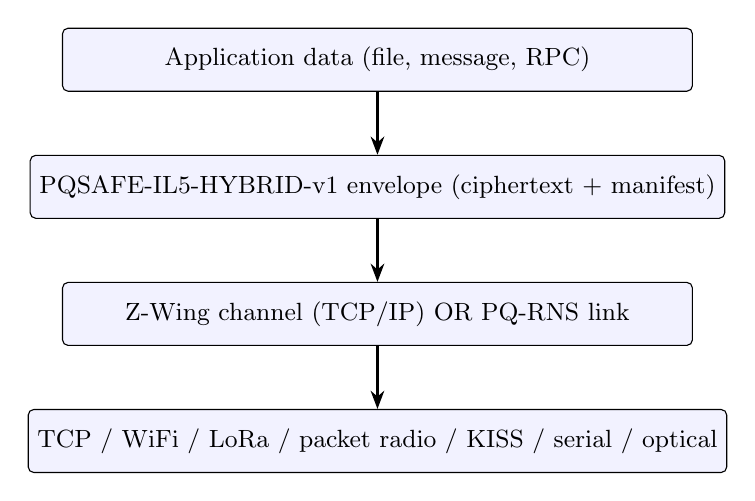
\begin{tikzpicture}[
  node distance=8mm and 14mm,
  every node/.style={font=\small},
  box/.style={draw, rounded corners=2pt, minimum height=8mm,
              minimum width=30mm, align=center},
  layer/.style={draw, rounded corners=2pt, minimum height=8mm,
                minimum width=80mm, align=center, fill=blue!5}
]
\node[layer]                       (app)   {Application data (file, message, RPC)};
\node[layer, below=of app]         (pqsafe){PQSAFE-IL5-HYBRID-v1 envelope (ciphertext + manifest)};
\node[layer, below=of pqsafe]      (chan)  {Z-Wing channel (TCP/IP) OR PQ-RNS link};
\node[layer, below=of chan]        (carrier){TCP / WiFi / LoRa / packet radio / KISS / serial / optical};

\draw[-Stealth, thick] (app)    -- (pqsafe);
\draw[-Stealth, thick] (pqsafe) -- (chan);
\draw[-Stealth, thick] (chan)   -- (carrier);
\end{tikzpicture}
\caption{Composition stack. PQSAFE envelope rides over either Z-Wing
(TCP/IP) or PQ-RNS (mesh / LoRa / packet radio). The carrier layer is
chosen at runtime; the envelope is identical.}
\end{figure}

\begin{itemize}[leftmargin=*,itemsep=0pt]
\item \textbf{PQSAFE} is the application-layer envelope. Every byte
  that leaves the sender is encrypted, signed, manifest-bound, and
  audit-anchored.
\item \textbf{Z-Wing} is the secure channel over TCP/IP. Provides
  endpoint authentication, replay protection, and hybrid PQ
  confidentiality.
\item \textbf{PQ-RNS} is the secure channel over non-IP carriers.
  Same role as Z-Wing but for mesh, LoRa, packet radio, etc.
\item The choice between Z-Wing and PQ-RNS is made by the application;
  the PQSAFE envelope doesn't care which carrier it rides.
\end{itemize}

% ===========================================================================
\section{Use cases}
\label{sec:usecases}

\subsection{Disaster recovery / off-grid mesh}

After an event that knocks out IP infrastructure (storm, cyberattack,
EMP), PQ-RNS over LoRa lets agencies continue to exchange CUI files
encrypted with PQSAFE. The PQ leg ensures that even a passive recorder
operating during the outage cannot retrospectively decrypt the
exchanged files when IP comes back online and the recordings can be
processed with future CRQCs.

\subsection{Contested EW environments}

In a contested electromagnetic environment, RNS's medium-agility
(LoRa, packet radio, optical, custom modems) makes it harder for an
adversary to deny service across all carriers simultaneously. The PQ
layer ensures that even traffic captured during the contest is
post-quantum secure.

\subsection{Validator gossip on degraded networks}

Lux primary-network validators that lose IP connectivity but retain a
LoRa or packet-radio backhaul to other validators continue to gossip
consensus messages via PQ-RNS. The QuasarCert wire format is
unchanged; the carrier moves underneath.

\subsection{Cross-agency air-gap bridges}

An air-gap can be bridged with a directional optical link or a
dedicated LoRa hop. PQ-RNS rides that hop with PQ confidentiality;
the air-gap policy enforces classification at the endpoint, not at
the wire.

\subsection{Out-of-band identity provisioning}

For PSK-hybrid mode (Section~\ref{sec:pq-rns}), long-term ML-KEM-768
public keys are exchanged through QR codes, signed PDFs, or a
trusted IP rendezvous. The PQ-RNS link then bootstraps with no
plaintext identity exchange over the constrained carrier.

% ===========================================================================
\section{Migration and compatibility}
\label{sec:migration}

\subsection{Mixed networks}

Native RNS and PQ-RNS coexist transparently. A PQ-capable node
advertises both classical and hybrid capabilities in its announce
frame. Classical-only nodes ignore the \texttt{pqrns} block and engage
classical link establishment; PQ-capable nodes detect each other and
upgrade to hybrid.

A \texttt{require: true} node refuses classical-only peers entirely,
which is what strict-PQ enclaves want: a misconfigured classical-only
peer in a strict-PQ enclave fails to link with any local peer rather
than silently falling back to classical.

\subsection{Migration to pure-PQ RNS}

Pure-PQ RNS is the explicit exit ramp:

\begin{enumerate}[leftmargin=*,itemsep=0pt]
\item \textbf{PQ-RNS-HYBRID-v1} (this profile): X25519 + ML-KEM-768,
  Ed25519 + ML-DSA-65. Production today.
\item \textbf{PQ-RNS-HYBRID-v2}: X448 + ML-KEM-1024,
  Ed448 + ML-DSA-87. High-assurance variant; same shape, larger
  parameters.
\item \textbf{PQ-RNS-PURE-PQ-v1}: ML-KEM-768/1024 only,
  ML-DSA-65/87 only (no X25519/X448, no Ed25519/Ed448). Activated
  when CNSA 3.0 (or equivalent) policy permits classical-curve
  removal in mesh deployments.
\end{enumerate}

Mixed-version operation is supported as long as both peers agree on a
version they both implement. The reference RNS implementation is not
expected to add PQ natively; the Lux PQ-RNS profile is the
interoperable extension.

% ===========================================================================
\section{What we don't do}

\begin{itemize}[leftmargin=*,itemsep=0pt]
\item Don't fork the RNS reference implementation.
\item Don't replace AES-256-CBC + HMAC-SHA-256 with a new AEAD unless
  the reference implementation does so first (preserves
  interoperability).
\item Don't add cipher-suite negotiation inside a profile. New
  capabilities are new profile versions, not parameters within a
  profile.
\item Don't claim PQ-RNS is "RNS" in protocol-conformance language.
  It is a Lux extension; the reference RNS implementation is the
  authoritative protocol definition. PQ-RNS is interoperable with
  native RNS by design; non-PQ nodes see PQ nodes as ordinary RNS
  peers.
\item Don't run pure-PQ RNS before the migration window closes.
  Lattice-only mode loses the X25519 fallback if a future
  lattice-specific attack appears.
\end{itemize}

% ===========================================================================
\section{Conclusion}

PQ-RNS is the post-quantum extension that lets Reticulum's
mesh-networking philosophy carry forward into the CRQC era without
losing what makes RNS uniquely useful: zero coordination, initiator
anonymity, half-duplex carriers, and operation on any wire from 5\,bps
to 1\,Gbps. The cost is one-off: a 9 KiB handshake per link, amortised
across the lifetime of that link. The benefit is permanent:
retrospective decryption of recorded sessions requires breaking both
the X25519 ephemeral half and the ML-KEM-768 ephemeral half of the
hybrid key exchange, and the long-term identity continues to verify
under both Ed25519 and ML-DSA-65.

Paired with Z-Wing for TCP/IP and PQSAFE for envelope encryption,
PQ-RNS completes the Lux end-to-end post-quantum stack: \emph{every
byte that leaves a Lux endpoint can be encrypted with NIST-standardised
hybrid primitives no matter what carries it.}

% ===========================================================================
\begin{thebibliography}{99}

\bibitem{rns-repo}
Mark Qvist et al. \emph{Reticulum Network Stack -- Reference
Implementation.} \url{https://github.com/markqvist/Reticulum}

\bibitem{rns-manual}
Mark Qvist. \emph{Reticulum Network Stack -- Manual.}
\url{https://markqvist.github.io/Reticulum/manual/}

\bibitem{rns-zen}
Mark Qvist. \emph{The Zen of Reticulum.}
\url{https://github.com/markqvist/Reticulum/blob/master/Zen\%20of\%20Reticulum.md}

\bibitem{fips203}
NIST. \emph{FIPS 203: Module-Lattice-Based Key-Encapsulation Mechanism
Standard.} August 2024.
\url{https://csrc.nist.gov/pubs/fips/203/final}

\bibitem{fips204}
NIST. \emph{FIPS 204: Module-Lattice-Based Digital Signature Standard.}
August 2024.
\url{https://csrc.nist.gov/pubs/fips/204/final}

\bibitem{fips205}
NIST. \emph{FIPS 205: Stateless Hash-Based Digital Signature Standard.}
August 2024.
\url{https://csrc.nist.gov/pubs/fips/205/final}

\bibitem{cnsa2}
NSA. \emph{Commercial National Security Algorithm Suite 2.0
(CNSA 2.0).} September 2022.

\bibitem{xwing2024}
Manuel Barbosa et al. \emph{X-Wing: The Hybrid KEM You've Been Looking
For.} IACR ePrint 2024/039;
IETF \texttt{draft-connolly-cfrg-xwing-kem}.

\bibitem{lp9701}
Lux. \emph{LP-9701: Reticulum Network Stack hybrid PQ profile.}
\url{https://github.com/luxfi/lps/blob/main/LPs/lp-9701-reticulum-network-stack.md}

\bibitem{luxzwing}
Lux Industries Inc. \emph{luxfi/zwing: Z-Wing post-quantum secure
channel + canonical X-Wing / hybrid-identity primitives.}
\url{https://github.com/luxfi/zwing}

\bibitem{luxpqrns}
Lux Industries Inc. \emph{luxfi/pqrns: PQ-RNS hybrid post-quantum
profile for the Reticulum Network Stack.}
\url{https://github.com/luxfi/pqrns}

\bibitem{pqsafe}
Lux Industries Inc. \emph{PQSAFE-IL5-HYBRID-v1: DoD-grade PQ envelope
encryption.}
\url{https://github.com/luxfi/papers/tree/main/pqsafe-il5}

\bibitem{rnode}
Mark Qvist. \emph{RNode: an open-source LoRa-based interface for
Reticulum.} \url{https://unsigned.io/rnode/}

\end{thebibliography}

\end{document}
